\chapter{Enfoque General}
\label{chapter:estrategia}

\section{Estrategia propuesta}
Con el fin de crear una aplicación que satisfaga los requerimientos mencionados anteriormente, se debe encontrar
un procedimiento que incluya desde obtener los datos relevantes de la web hasta llevarlos a un estado que permita una 
explotación satisfactoria. 

El procedimiento debería incluir los siguientes pasos  

\begin{description}
\item[Selección de vocabularios ] Tanto la recolección como la publicación de datos en la web semántica involucra la elección del o de los vocabulario/s que mejor modelen el dominio de problema, con la excepción que para su publicación existe la posibilidad de desarrollar uno propio que se ajuste correctamente en caso de que no se encuentre uno existente. 
\item[Recolección  ] Proceso que comprende dos tareas (Búsqueda y Obtención) en el cual se intenta conseguir los datos deseados, los cuales se encuentran dispersos en la web y para ello pueden utilizarse múltiples herramientas y servicios web.
\item[Extracción y almacenaje de los datos] Se le aplica estos dos pasos a los datos crudos obtenidos en la web para poder tener la información semántica y descartar el resto en un formato mucho mejor procesable.
\item[Evaluación de Calidad de los Datos] Se evalúa si los datos poseen la calidad mínima necesaria para crear una aplicación que satisfaga a los requerimientos.
\item[Curado de los Datos] Intentar corregir los problemas de calidad de los datos encontrados en el paso anterior. Siempre y cuando sea posible y viable.
\item[Integración de los datos] Este puede ser el proceso más costoso pero también el más importante, en el cual se intenta unificar e interconectar la información para que pueda ser aprovechable. Existen distintos niveles de integración más simples o más complejos.
\item[Publicación del Dataset Curado] El dataset ya con una calidad teóricamente superior y un estado mucho más aprovechable que el que se encontraba en un primer momento se deja a disposición de todos de forma online.  
\item[Explotación del Dataset] Se construye una aplicación que en base a los requerimientos utilice el dataset. 
\end{description}

\begin{figure}
    \centering
    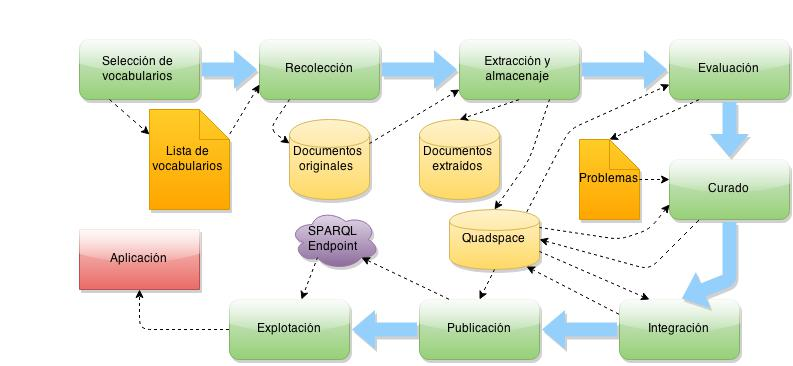
\includegraphics[width=0.8\textwidth,natwidth=610,natheight=642]{proceso}
    \caption{Flujo completo del procedimiento}
\end{figure}

\begin{framed}
\textcolor{red}{acá sería bueno incluir un diagrama que muestre el pipeline. En la lista de arriba con un párrafo se explica cada paso. Luego, en las secciones que sigue se analiza mas cada paso, pero se lo plantea como un problema.. se analizan los retos; entonces los capítulos 4 a 9, explican como los resolviste. Alternativamente, se puede hablar menos acá, solo lo suficiente para que se entienda la estrategia general, y luego en los capítulos 4 a 9 se analiza el problema en detalle y se propone la solución. Con esta ultima forma, todo lo que se refiere a los vocabularios quedaría en el capitulo 4 y no acá. Puede ser mejor.}
\end{framed}

\section{Selección de vocabularios}

\noindent Seleccionar un vocabulario implica analizar varios aspectos del mismo, no sólo su definición e implementación, sino también el uso práctico dado por sus usuarios. 
En primer lugar se debe comprobar que los nombres de las propiedades que posee sean correctamente auto-explicativas. Supongamos por ejemplo que existe un ítem con un rating agregado modelado por una ontología que posee las siguientes propiedades:

\begin{enumerate}
\item minrating
\item ratingValue
\item countRating
\end{enumerate}


\noindent Las dos últimas propiedades resultan fácilmente identificables, ratingValue se trata del promedio de puntaje, y ratingCount 
la cantidad de puntajes que le fueron otorgados, pero la propiedad minRating podría generar distintas formas de interpretación, 
alguien podría suponer que se trata del valor mínimo que fue adquirido por un usuario, o el valor mínimo que un usuario puede 
otorgar. Y muchas veces la documentación de la ontología (si es que existe) no es suficiente.
\\\\
\begin{framed}
\textcolor{red}{Explicar que en realidad uno no elige ``un'' vocabulario sino que la información podría expresarse combinando términos de varios vocabularios. Dejar claro que no es lo mismo elegir el/los vocabulario/s en el que uno va a publicar que decidir cuales son todos los vocabularios que uno va a considerar al buscar información publicada por otros - dar un ejemplo}
\end{framed}

\begin{framed}
\textcolor{red}{Este párrafo que sigue no se entiende; aclarar que sería cubrir las necesidades mínimas de los casos de uso.}
\end{framed}

\noindent Luego se deberá analizar si existen las propiedades para cubrir las necesidades mínimas de los casos de uso. Esto significa que pueda modelar 
toda la información que más adelante será requerida. Por ejemplo, si se quiere construir una aplicación que compare autos, al momento 
de elegir un vocabulario que modele autos, es necesario que contenga ciertas propiedades que puedan expresar información  para determinados 
casos de uso, como comparar cantidad de puertas, lo que requeriría que el vocabulario elegido contenga una propiedad que exprese la cantidad 
de puertas del auto.
\\\\
Es posible que ante una aplicación muy extensa, con casos de uso muy complejos, no se consiga un vocabulario con propiedades tan abarcativas 
que puedan cubrir todos los casos de uso. 

Para esto, se puede aprovechar que las propiedades de un vocabulario, no necesariamente tienen que ser utilizadas estrictamente dentro del mismo.
Lo único que debe respetarse es el dominio y rango de cada una, si no se explicita, puede utilizarse en otros vocabularios.

Goodrelations\cite{Hepp2008} es un ejemplo del uso de propiedades de múltiples vocabulairos para crear uno nuevo.
\\\\
Y por último se debería intentar buscar ejemplos reales que muestren el uso que le dieron los usuarios a la ontología, para 
determinar qué propiedades están incorrectamente interpretadas o también para los casos donde las propiedades que se encuentren 
en desuso.
\\\\
Con estas precauciones en mente se puede emprender la búsqueda, que podría tener como comienzo búsquedas en  search engines. 
Existen dos buscadores específicos para esta tarea:

\subsection{Linked Open Vocabulary (LOV)}

\cite{Vandenbussche2012} Proporciona una plataforma técnica de búsqueda y evaluación de calidad sobre un dataset extraído de linked data cloud que contiene descripciones de vocabularios RDFS 
y ontologías OWL. Esas descripciones están en forma de metadatos y pueden ser generados tanto por los autores de los vocabularios como por curadores de LOV.
Posee además de la búsqueda las funciones de estadística o sugerencia.

Actualmente el dataset está integrado por 475 namespaces distintos que contienen una media de 10 clases y 20 propiedades, siendo schema.org el más grande de ellos.

\subsection{Vocab.cc}
Vocabcc es un proyecto opensource que permite a los desarolladores de RDF realizar búsquedas de vocabularios de Linked Data.

Para facilitar la decisión de seleccionar un vocabulario deseado, proporciona además información estadística de cada uno sobre el dataset Billon Triple Challenge (BTCD)\cite{btc-2012}. 
 Esta información incluye el número de apariciones globales de la URI dada en el BTCD, así como el número de documentos dentro de la BTCD, que contiene el URI dado. Estos números permiten una clasificación de propiedades y clases, respectivamente, con respecto a su uso. También se proporciona información acerca de la posición de una URI dada en estos rankings.

Los desarrolladores pueden buscar las URIs con queries arbitrarias o búsquedas de URIs específicos (prefijos comunes se resuelven automáticamente con datos de prefix.cc).

Para permitir una fácil integración de la funcionalidad vocab.cc, toda la información está disponible como RDF y se puede acceder como Servicio Vinculado.

\begin{framed}
\textcolor{red}{Una vez definidos el/los vocabularios a utilizar, se debe proceder a recuperar información disponible en la web; a eso llamamos ``Recolección''}
\end{framed}

\section{Recolección}
\label{section:recoleccion}
%Como se mencionó antes, la web contiene grandes cantidades de documentos publicados con información semántica. Pero la tarea
de encontrarlos, con el agregado de que sólo una pequeña porción de ellos será relevante para los requerimientos no es trivial
en lo absoluto debido a la inmensidad del universo en el que se encuentran. La forma de llevar a cabo este objetivo está 
atada al hardware disponible, tanto para almacenar los datos, como para el tiempo que va a emplear la ejecución de esta 
tarea. \\
Dado que las bases de datos semánticas sólo almacenan información en forma de tripletas o cuadrupletas, los documentos encontrados 
deberán someterse a un proceso de extracción que seleccione las sentencias HTML y las convierta a alguno de los lenguajes que soportan  
tripletas o cuadrupletas. Para esto existen múltiples herramientas.\\
Una vez transformados los documentos HTML a documentos semánticos puede construirse la base de datos semántica con la información 
recolectada.\\
Como se mencionó antes, la web contiene grandes cantidades de documentos publicados con información semántica. Pero la tarea
de encontrarlos, con el agregado de que sólo una pequeña porción de ellos será relevante para los requerimientos no es trivial
en lo absoluto debido a la inmensidad del universo en el que se encuentran. La forma de llevar a cabo este objetivo está 
atada al hardware disponible, tanto para almacenar los datos, como para el tiempo que va a emplear la ejecución de esta 
tarea.  
\\\\
Dado que las bases de datos semánticas sólo almacenan información en forma de tripletas o cuadrupletas, los documentos encontrados 
deberán someterse a un proceso de extracción que seleccione las sentencias HTML y las convierta a alguno de los lenguajes que soportan  
tripletas o cuadrupletas. Para esto existen múltiples herramientas. 

Una vez encontrados, descargados y transformados los documentos HTML a documentos semánticos puede construirse la base de datos semántica 
con la información recolectada. 
\\\\
Estos son los cuatro pasos necesarios para lograr tener el dataset semántico con el cual se puede empezar a trabajar. Cada uno de ellos 
posee distintas alternativas para su realización, algunas se describirán a continuación 


%\input{opcionesBusqueda}
\\
\input{opcionesDescarga}
\\
\input{opcionesTransformación}
\\
\input{opcionesAlmacenaje} vacio

\subsection{Búsqueda}
%\input{opcionesBusqueda}
\textcolor{red}{OJO: ESTO ESTABA EN EL ARCHIVO busqueda.tex no en el opcionesBusqueda}


La forma de ejecución de esta tarea dependerá de algunos aspectos:
\begin{itemize}
\item Recursos de hardware disponibles

\item Cantidad y calidad de la información requerida

\item El grado de atemporalidad mínima tolerable en los datos

\end{itemize}

El primer paso para realizar la recolección es intentar responder la siguiente pregunta: \textit{¿Dónde encuentro la informanción?}

Una vez seleccionados los vocabularios, se necesitará obtener fuentes de datos que contengan sus datos publicados en los vocabularios previamente seleccionados.
 \\\\
Para lograrlo se podrá utilizar como punto de partida:
\begin{description}
\item[Sitios indexadores:] Son algunos sitios que disponen de un dataset muy grande procesado con documentos indexados, que ofrecen consultar dicho 
dataset a travez servicios web. Generalmente proveen una API donde se pueden consutlar los datos mediante distintos grados de flexibilidad.

Sindice, LOD cloud cache y UriBurner son algunos ejemplos de estos sitios. Se puede utilizar entocnes, dichos servicios web a fin
de obtener una lista de URLs en las cuales se cree que contendrán la información necesaria.

\item[Sitios autoritativos:] Son sitios conocidos que generan información relevante y la publican en las ontologías y vocabularios 
seleccionados. Ejemplos aplicados al caso de estudio podrían ser IMDB (que publica reviews de películas bajo el vocabulario schema), o Rottentomatoes
(que hace lo mismo pero no solo con películas). Se podrán utilizar entonces estos sitios como punto base para un posible crawling.

\item[Catálogos de enpoints:] Son catálogos provistos por algunos sitios que mantienen una lista actualizada de SPARQL endpoints 
junto con el estado de disponibilidad en el que se encuentran. Por ejemplo los sitios http://labs.mondeca.com/sparqlendpointsstatus/ y 
http://www.w3.org/wiki/SparqlEndpoints que este último además provee detalles sobre la información de los mismos.

Consultar estos sitios entonces generará una lista de endpoints SPARQL los cuales se podrían utilizar para pedir la información necesaria.

\item[Volcados de datos:] Son datasets muy grandes que fueron el resultado de un web crawling, los cuales están disponibles para su descarga 
y se pueden utilizar para procesarlos y obtener los datos requeridos. El más importante es http://challenge.semanticweb.org/2014/ .
\end{description}
\subsection{Obtención}

Este paso está directamente relacionado con el anterior, dado que la estrategia de obtención fue planeada con anterioridad, según 
cuál sea la seleccionada, habrá sido la opción ejecutada en el paso anterior.
\\\\
Para este paso se tienen las siguientes estrategias:
\begin{description}
\item[Web Crawling:] Realizar un crawling partiendo de unas pocas URLs seleccionadas en el paso anteiror. Obtenidas de sitios autoritativos.
Existen formas distintas de hacer web craling, dependiendo del nivel de profundidad en el cuál se recorrerá la web, podría también utilizarse los 
sitios indexadores, SPARQL queries, o motores de búsqueda para obtener una lista de URLs que contienen la información deseada, y luego realizar un crawling de profundidad uno sobre cada url.
Hacer crawling con profundidades muy grandes requiere de una algoritmia mucho más compleja para evitar loops, y también de muchos más recursos de hardware, pero se podrá obtener mucha más información.

\item[De-referenciamiento de URIs:] Igual al web crawling, pero exclusivo de documentos semanticos NO embebidos, ya escritos en un formato nativo de la web semántica como RDF, turtle, n-Triples, etc.
Luego la profundidad puede continuarse realizando lo que se llama un ''follow your nose'', que se realiza de-referenciando los documentos que son objeto de la propiedad owl:sameAs, o rdf:seeAlso.

\item[Descarga de las respuestas de las APIs:] Este es otro caso del uso de lso sitios indexadores, SPARQL queries, o motores de búsqueda. Pero en lugar de 
que la información  utilizada sean simpelmente las URL de los documentos, se utilizará también la ifnromación cacheada de dichos documentos y evitarse un crawling.
Como desventaja se puede tener información desactualizada, pero como ventaja se podrá obtener información que ya no esté disponible. Todo dependerá de lo que se busque obtener.
La información obtenida de estas APIs ya debería encontrarse en un formato de la web semántica por l oque no requerirá tampoco una futura extracción.

\item[Procesamiento de grandes volcados:] Este paso requiere de la utilización de recursos minímos de hardware, ya que estos volcados suelen tener volúmenes de varios teras de información, y para procesarlos se requerirá 
de mucha RAM, memoria secundaria y microprocesador.
La idea de este paso es inspeccionar el volcado o bienpara obtener la URL de los documentos con la información deseada, para luego realizar un crawling de profundidad 1, 
o directamente utilizar la información contenida en el volcado.
Esta opción enrealidad es una suma de un paso intermedio con las demás opciones de este paso ya que se estaría realizando el trabajo que hacen los indexadores, que es procesar grandes volúmenes de datos.
\end{description}

\section{Extracción y almacenaje}
\label{section:extraccion}
Una vez que se logró encontrar la información requerida en la web y contener una copia local, se necesita darle un mínimo procesamiento a determinados datos.
Específicamente a aquellos que estén en un formato de información semántica embebida, que requeriran un proceso de extracción para luego ser almacenados en un triplestore.


\subsection{Extracción}

Esto significa, parsear el documento HTML, que como mensionamos anteriormente puede contener información semántica en formato RDF-a, microformatos o microdatos, buscando 
la información semántica para luego generar un documento RDF (o de otro lenguaje de tripletas puro) que represente esa información semántica encontrada en tripletas que puedan ser almacenadas bajo un triplestore.
\\\\
Si bien podría escribirse manualmente un algoritmo que realice esta tarea, existen muchas herramientas que lo hacen, por lo que es recomendable la utilización de alguna de ellas.
\\\\
Los extractores más utilizados son los siguientes:
\begin{itemize}
\item getSchema: Es una herramienta online que se utiliza a travez de una API Restful para extraer documentos con microdatos. Como respuesta se obtendrán documentos semánticos 
con la información extraída en formatos N-Triples, JSON, o N3. 
Es una herramienta rápida y eficaz pero sólo sirve para microdatos.

\item RDF Translator: Funciona también a travez de una API restful, y además de soportar también docuemntos con formato RDF-a, proveé la funcionalidad de transformar los documentos en sentido inverso, 
(de tripletas a información semántica embebida en HTML). 
También está la posibilidad de descargarse la librería y correr el algoritmo localmente.

\item Any23: Una herramienta muy potente y completa que cuenta con una comunidad que lo actualiza constantemente. Al igual que las anteriores se puede utilizar de forma online a travez 
de una API restful. Tiene como ventaja que soporta también microformatos. Es el extractor utilizado por Sindice. 
También está disponible en forma de librería para utilizar localmente.

\item Data Linter:Es una herramienta online que parsea documentos RDF-a, microdatos y JSON-LD.  
Muy útil para analizar documentos, ya que dispone de varias ventajas: 

Presenta la información organizada en tablas anidadas que son mucho más amigables para un análisis humano. 

Posee un mecanismo de inferencia que alerta cuando se viola la sintaxis de los vocabularios.

Como contrapartida, la información retornada por la herramienta es en texto plano. Por lo que no puede ser utilizado en un triplestore.

\end{itemize}

\subsection{Almacenaje}

Con la información recolectada de internet en forma de tripletas (o cuadrupletas) ya puede ser almacenada conjuntamente en un triplestore. 

Se disponen de muchas opciones de triplestores en la actualidad, algunos pagos y otros gratuitos. Cada uno con ventajas en algunos aspectos y desventajas en otros.

Muchos son librerías que forman parte de un framework, además algunos mapean tripletas a otros motores de base de datos como por ejemplo MYSQL o POSGRE.
\\\\
Algunos posibles triplestores pueden ser
\begin{itemize}
\item TDB: Componente del framework Jena, que puede ser accedido mediante linea de comandos o a travez de la API de jena. Almacena tanto tripletas como cuadrupletas, y las almacena en varios archivos donde cada uno indexa los datos de distintas formas. Tiene una muy aceptable performance pero pequeños errores en su uso pueden corromper la información facilmente.

\item SDB: Al igual que TDB es un componente de Jena, pero que no almacena la información como archivos en el disco, sino que mapea los datos a un motor de bases de datos subyacente como MYSQL y POSGRE. Su performance está atada a dicho motor de bbdd subyacente pero por lo general no suele dar buenos resultados. 

\item Sesame triplestore: Componente del framework Sesame, que tiene la opción de almacenar la información en disco o en memoria. Lo que puede significar un improtante beneficio para quienes requieran performance elevada en queries. Soporta no solo SPARQL sino también SeRQL. Tiene además la ventaja de poder integrar Alibaba, que es un mapeador de calses de Java a ontologías RDF.
\end{itemize}

\noindent En el capítulo 6 de \cite{Bizer2001} se observan los siguientes resultados comparativos entre las distintas bases de 
datos semánticas.

\begin{itemize}
\item To load 100m triples of evaluation data:
 \begin{description}
     \item[Sesame:] 3 days 6 hours
     \item[Jena TDB:] 1.5 hours
     \item[Jena SDB:] 1 day 15 hours
 \end{description}
\item Complex Query Mixes per Hour (rate of query answering -- higher = better) for 1M triples:
 \begin{description}
     \item[Sesame:] 18,094
     \item[Jena TDB:] 4,450
     \item[Jena SDB:] 10,421
 \end{description}
\item Complex Query Mixes per Hour for 25M triples:
 \begin{description}
     \item[Sesame:] 1,343
     \item[Jena TDB:] 353
     \item[Jena SDB:] 968
 \end{description}
\item Complex Query Mixes per Hour for 100M triples:
 \begin{description}
     \item[Sesame:] 254
     \item[Jena TDB:] 81
     \item[Jena SDB:] 211
 \end{description}
\item Simple Query Mixes per Hour for 1M triples:
 \begin{description}
     \item[Sesame:] 38,727
     \item[Jena TDB:] 15,842
     \item[Jena SDB:] 15,692
 \end{description}
\item Simple Query Mixes per Hour for 25M triples:
 \begin{description}
     \item[Sesame:] 39,059
     \item[Jena TDB:] 1,856
     \item[Jena SDB:] 4,877
 \end{description}
\item Simple Query Mixes per Hour for 100M triples:
 \begin{description}
     \item[Sesame:] 3,116
     \item[Jena TDB:] 459
     \item[Jena SDB:] 584
 \end{description}
\end{itemize}
        

No sólo se debería elegir el triplestore en cuanto a su performance, su facilidad de uso y flexibilidad también es un aspecto muy importante a evaluar.

%\input{opcionesDescarga}
%input{opcionesTransformación}
%input{opcionesAlmacenaje}

 

\section{Evaluación de Calidad de los Datos} 
\label{section:evaluacion}
Como sabemos los reviews son creados por usuarios que en su mayoría no están familiarizados con el desarrollo de una 
aplicación, esto causa que una parte muy significativa del contenido publicado no esté de la forma adecuada para ser procesado. 
La falta de calidad en el contenido publicado puede deberse tanto a errores por parte del usuario como por parte del publicador.

El publicador deberá asegurarse que los datos respeten rigurosamente las ontologías en las cuales se publican.
\\\\
El sitio web en el cual el usuario se encuentre realizando el review deberá guiarlo en todo lo posible para lograr que la evaluación
quede en un formato adecuado.

Aunque también existen muchos problemas que no dependen del sitio web, generalmente errores semánticos de calidad, donde lo 
redactado esta hecho de forma inconsistente o insuficiente.
\\\\
Este paso entonces tiene por objetivo encontrar todos los problemas de calidad que pueda haber en el dataset que acaba de 
ser descargado y extraído y que generen inconvenientes para una posterior integración/explotación.
\\\\
La estrategia se divide en dos partes, una formal y otra informal.
\\\\
La formal se encuentra ligada a la detección de errores sintácticos en el dataset, que son generalmente causados por una mala utilización del vocabulario (Aunque también suelen aparecer problemas causados por malas definiciones de los vocabularios)

El ejemplo típico de este tipo de error es el uso incorrecto del dominio o rango de una propiedad. 

Encontrar este tipo de errores no es una tarea demasiado compleja, disponiendo de los vocabularios se puede hacer inferencia sobre el dataset y determinar automáticamente los errores sintácticos.
\\\\
Y luego se encuentra la estrategia informal, que intenta encontrar los problemas semánticos del dataset, para los cuales resulta extremadamente difícil su detección automatizada.

Un ejemplo de este caso es la falta de información precisa necesaria para identificar un ítem, por ejemplo poner ``batman'' como nombre, siendo esta la única forma de identificarlo. Como sabemos batman puede referirse a muchos ítem distintos y se necesita un nombre más preciso para su identificación.
Este problema haría más dificultosa una posible integración, ya que no sería tan simple identificar cuales reviews hablan de los mismos ítems.

Otro ejemplo es el de la inconsistencia en la información provista, si por ejemplo se establece schema:Book como tipo de ítem pero el nombre del ítem es ``Samsung SyncMaster 753s'' claramente es el caso de un tipo incorrecto, ya que hay una propiedad que sólo tendría sentido si se tratara de un schema:Product.
Este último error modificaría el correcto funcionamiento de una posible aplicación resultante además de interferir en la integración. Ya que si esa aplicación por ejemplo, lista reviews según el tipo de ítem, cuando un usuario busque reviews de libros, se encontraría con el review de un monitor.
\\\\
Estos últimos errores suelen ser muy difíciles de encontrar y prácticamente imposibles de detectar mediante búsquedas automáticas.

Para lograrlo se requiere observar humanamente el vocabulario y reflexionar sobre el mismo, deduciendo errores que podrían aparecer, también ayudaría mucho observar resultados de estadísticas sobre el uso de propiedades en el dataset.
\\\\
Existen frameworks para realizar estas operaciones.

%Curado de los Datos\\
En el paso anterior se describieron los problemas en la calidad del dataset que tendrán un impacto en la aplicación resultante, 
o que, podrían limitar o imposibilitar la realización de la misma. Dichos problemas pueden ser muchos, y algunos muy difíciles
de solucionar, será parte entonces del proceso, reconocer aquellos que su resolución sea viable y además encontrar la forma de 
implementarla.\\
Cabe destacar que el proceso de evaluar el dataset en búsqueda de problemas y implementar soluciones es iterativo, debido a que 
una mejora puede conllevar a nuevos problemas.\\
\section{Curado de los Datos}

En el paso anterior se describieron los problemas en la calidad del dataset que tendrán un impacto en la aplicación resultante, 
o que, podrían limitar o imposibilitar la realización de la misma. Dichos problemas pueden ser muchos, y algunos muy difíciles
de solucionar, será parte entonces del proceso, reconocer aquellos que su resolución sea viable y además encontrar la forma de 
implementarla.
\\\\
Cabe destacar que el proceso de evaluar el dataset en búsqueda de problemas y implementar soluciones es iterativo, debido a que 
una mejora puede conllevar a la detección de nuevos problemas.

%Integración de los datos\\
Los datos recolectados fueron generados por distintos usuarios, en múltiples sitios y bajo distintas ontologías y estándares.
Estos aún curados, necesitan un último paso para poder realizar una explotación, y es la integración.\\
Este gran y dificultoso proceso abarca cualquier operación que intente dar una visión más unificada de la información. Este
proceso puede tener distintos niveles y aspectos a integrar, como podría ser por ejemplo, unificar las ontologías de los reviews, o bien
en una nueva ontología de review, o bien en una ya existente, para lograr tener información semánticamente más parecida. Ya 
que este proceso puede ser muy dificultoso, habrá que ver en base a los requerimientos, qué aspectos de los datos se integrarán.\\
Una vez realizada la integración mínima necesaria par also requerimientos, el dataset ya estará listo para su explotación.

\section{Integración de los datos}
\label{section:integracion}
\begin{framed}
\textcolor{red}{Esto va acá o es parte de Explotación?}
\end{framed}

Los datos recolectados fueron generados por distintos usuarios, en múltiples sitios y bajo distintas ontologías y estándares.
Estos aún curados, necesitan un último paso para poder realizar una explotación, y es la integración.
\\\\
Este gran y dificultoso proceso abarca cualquier operación que intente dar una visión más unificada de la información. Este
proceso puede tener distintos niveles y aspectos a integrar, como podría ser por ejemplo, unificar las ontologías de los reviews, o bien
en una nueva ontología de review, o bien en una ya existente, para lograr tener información semánticamente más parecida. Ya 
que este proceso puede ser muy dificultoso, habrá que ver en base a los requerimientos, qué aspectos de los datos se integrarán.
\\\\
Una vez realizada la integración mínima necesaria para los requerimientos, el dataset ya estará listo para su explotación.

\section{Publicación del Dataset Curado}

Existen varias maneras de publicar el dataset, y la elección de una en particular dependerá tanto de para qué se podría utilizar el dataset en el futuro como
de los recursos de tiempo/hardware/económicos que se esté dispuesto a gastar.
\\\\
Una posible solución muy barata y simple es generar un volcado de la base de datos, comprimirlo y subirlo a un hosting de archivos como Mega. Cualquier usuario podría descargarse entonces la base de datos y utilizarla de la forma que más le convenga.
Tendría el problema en ese caso de no serle útil a usuarios con pocos conocimientos sobre esta tecnología, o que no posean demasiados recursos de hardware, o tiempo.

Una solución un poco más costosa es utilizar un servidor (ya sea propio, pago, o simplemente una pc), y crear un SPARQL Endpoint accesible mediante la web.
Esta última opción puede implementarse utilizando algúnas herramientas:
\begin{description}
\item [Fuseki:] SPARQL endpoint que utiliza el protocolo SPARQL mediante HTTP con estilo REST. Tiene una performance aceptable y la ventaja de ser muy sensilla su instalación y puesta en marcha. Se puede directamente utilizar un volcado de TDB.

\item [Virtuoso Server:] Middleware que incluye no solo un endpoint, sino también un motor de base de datos, un server, una aplicación web y todo lo necesario para publicar los datos en la web. Puede ser muy útil pero su instalación y puesta en marcha no es trivial. Y requiere la adquisición de una licencia para su uso.

\item [ARQ:] Componente de Jena que funciona como query engine, y puede ser utilizado para armar el endpoint manualmente, eso singifica realizar a mano la aplicación web.
\end{description}
\section{Explotación del Dataset}
\label{section:explotacion}
\begin{framed}
\textcolor{red}{Acá es donde efectivamente se discute que implica cubrir los requerimientos de la aplicación . Puede ser que acá tambien te refieras a como la forma en la que querés explotar los datos impacta en las fases anteriores. Incluso, habría que pensarlo, en este capitulo tal vez conviene primero hablar de explotación y luego de las otras fases - porque explotación determina mucho que es lo que vas a mirar en las fases anteriores, ¿no?}
\end{framed}

<<<<<<< HEAD
 Finalmente 
=======
\noindent Por último se llega al paso de explotación. 
\\\\
La forma en la que se proceda a implementarlo depende de múltiples factores que dependerán 
de los recursos de hardware disponibles, el tiempo de desarrollo que se deseé emplear y 
la calidad del dataset obtenido en los pasos anteriores.
\\\\
En general, cualquier aplicación resultante será correcta si logra respetar los requerimientos.
\\\\
El único punto a tener en cuenta es el de elegir correctamente un tipo de sistema de recomendación 
de manera que se pueda aprovechar de la mejor forma posible la información existente en el dataset. \\
Por ejemplo, si el dataset no contiene demasiados datos descriptivos de los ítems, no sería 
conveniente utilizar un sistema de recomendación basado en contenido, ya que la aplicación resultante 
no funcionaría de una forma muy útil.
De la misma forma que si dispone una gran cantidad de datos acerca de los autores, debería considerarse 
escoger un enfoque colaborativo para aprovechar de la mejor manera el dataset.
\\
\\
Teniendo eso en consideración, las herramientas/tecnologías/lenguajes/etc utilizados para su 
construcción y desarrollo.
>>>>>>> 49478991009a94744fb73d7dbf44ca15cd0cce27

